 
\ifx\synctex\undefined\else\synctex=1\fi

\documentclass[b5paper,11pt]{book}

\usepackage[utf8]{inputenc}
%% (FMu) uzywamy \lw do napisania l z kreska, bo potem cos
%% przedefiniowuje \l na \lambda. To nie jest eleganckie,
%% ale dziala. To samo dla czeskiego hacka (np. w Cerny)
\let\lw\l  
\let\hacek\v

\usepackage{amsfonts}
\usepackage[fleqn]{amsmath} %fleqn does left allignment of display formulas
\usepackage{amssymb,amsmath}
\usepackage{amsthm}
\usepackage{graphicx}
\usepackage{xspace}
\usepackage{todonotes}
\usepackage{mathbbol}
\usepackage{enumerate}
\usepackage{comment}
\usepackage{enumitem}
\usepackage{hyperref}
\usepackage{bookmark}
\usepackage{nameref}
\usepackage{ifthen}
\usepackage{algorithm}
\usepackage[noend]{algpseudocode}
\usepackage{tikz}
\usepackage[normalem]{ulem}
\usepackage[all]{xy}
% \usepackage{mdframed} 
\usepackage{fancyhdr}
\usepackage{pdfpages}
\usepackage{mathtools}


\RequirePackage[osf,sc]{mathpazo}
\usepackage[mathcal]{euscript}




% MACROS GENERATING THE GENERAL FLOW OF EXERCISES

% \setlist[itemize]{leftmargin=15pt, labelsep=5pt}

%\usepackage[parfill]{parskip}

% General list of sub-exercises, to be redefined soon...
\newenvironment{exEnum}
	{
	\begin{enumerate}}
	{\end{enumerate}}

% Enumerate list of EQUIVALENT STATEMENTS (!)
\newenvironment{exEnumEquiv}
	{
	\begin{enumerate}[label={\makebox[1em][c]{{\upshape({\itshape\alph*})}}},ref=({\itshape\alph*})]}
	{\end{enumerate}}

% Enumerate list of sub-exercises in the statement of problem
\newenvironment{exEnumStatement}
	{
	\begin{enumerate}[label={\upshape(\arabic*)},ref=(\arabic*)]}
	{\end{enumerate}}

% Enumerate list of sub-exercises in the solution of a problem
\newenvironment{exEnumSolution}
	{\mbox{}% 
	\begin{enumerate}[label=\textbf{\upshape\hyperref[\exRef]{\arabic{exnumber}}$\,$(\arabic*)}\hspace{3pt},ref=\arabic{exnumber}$\,$(\arabic*),%
		leftmargin=0pt,%
		itemindent=0pt,%
		labelsep=0pt,%
		align=left,%
		listparindent=\parindent, %
		parsep=0pt]
 % \setlist[itemize]{leftmargin=*,labelsep=5pt}
 \setlist[itemize]{leftmargin=\itemizemargin,labelsep=\itemizelabelsep}
 % \setlist[itemize]{leftmargin=\itemizemargin,labelsep=5pt}
	}
	{\qedhere\end{enumerate}}


%macros for manipulation of toc
\newcommand{\nocontentsline}[3]{}
\newcommand{\tocless}[2]{\bgroup\let\addcontentsline=\nocontentsline#1{#2}\egroup}
%usage:  \tocless\section{bla} or  \tocless\subsection{bla} 

%the following solution is taken from https://tex.stackexchange.com/questions/326412/multiple-page-numbers-on-element-of-toc
% the goal is to have two numbers in one row of the table of contents
\renewcommand\thechapter{\arabic{chapter}}
\renewcommand\thesection{\arabic{chapter}.\arabic{section}}
\renewcommand\thesubsection{\arabic{subsection}}


\makeatletter
\renewcommand{\@pnumwidth}{1cm}
\makeatother



\newcommand{\twonumbers}[2]{\hfill\makebox[0em][r]{#1}\makebox[1.2cm][r]{#2}}

\newcommand{\problems}[1]{%
\let\realsection\section%
\let\realchapter\chapter%
\newcommand{\pagebreaksol}{} %% Do nothing in this part.
%\renewcommand\addcontentsline[3]{}%
\renewcommand{\chapter}[1]{%
  \cleardoublepage%
  \thispagestyle{empty}%  
  \pdfbookmark[chapter]{##1}{chapter.\thechapter}%  
  \realchapter{##1}\label{section.\thesection}%
  \thispagestyle{empty}%
  \label{chapter.\thechapter}%
}%
\renewcommand{\section}[1]{%there is a problem when there is a pagebreak just before the section, then the bookmark points to the previous page
  \pdfbookmark[section]{##1}{section.\thesection}%  
  \realsection{##1}\label{section.\thesection}%
}%
\cleardoublepage%
\thispagestyle{empty}%
\pdfbookmark[part]{#1}{part.\thepart}%
\tocless\part{#1}%
\thispagestyle{empty}%  
}

\newcommand{\solutions}[1]{%
  \cleardoublepage%
  \thispagestyle{empty}%  
  \pdfbookmark[part]{#1}{part.\thepart}%  
  \part{#1}% 
  \thispagestyle{empty}%
  \renewcommand{\pagebreaksol}{\pagebreak}
  \renewcommand\addcontentsline[3]{}
    % todo: 
    % (1) if ##2 is 'chapter' then the pageref should be to chapter.\thechapter
    % (2) \thepage should be a hyperlink
%    \addtocontents{##1}{\protect\contentsline{##2}{##3}{\twonumbers{\pageref{section.\thesection}}{\thepage}}{section.\thesection}}%
  %}%
  \renewcommand{\chapter}[1]{%
    \cleardoublepage%
    \thispagestyle{empty}%  
    \pdfbookmark[chapter]{##1}{sol.chapter.\thechapter}%    
    \realchapter{##1}\label{sol.section.\thesection}%
    \thispagestyle{empty}
    \label{sol.chapter.\thechapter}%
  }%
  \renewcommand{\section}[1]{%
    \pdfbookmark[section]{##1}{sol.section.\thesection}%    
    \realsection{##1}\label{sol.section.\thesection}%
  }%
  % 
  \renewcommand{\assList}{FALSE}%
  \setcounter{chapter}{0}%
}
%%%%%%%%%%%%%%%%%%%%%%%%% end of toc macros


\theoremstyle{definition}

\newcommand{\exRef}{}

\newtheorem{exStatement}{Problem}

\theoremstyle{plain}%

\newtheorem{exSolution}{Problem}

\newcounter{exnumber}

\newcommand{\exercise}[3]{
\ifthenelse{\equal{\assList}{TRUE}}{
\let\exEnum\exEnumStatement%
\let\endexEnum\endexEnumStatement%
\setcounter{exnumber}{\value{exStatement}}%
\stepcounter{exnumber}%
\renewcommand\theexStatement{\hyperref[sol:#1]{\arabic{exnumber}}}%
\renewcommand{\assBody}{TRUE}%
\begin{exStatement}
\label{#1}
#2
\end{exStatement}
\renewcommand{\assBody}{FALSE}%
}{%





\let\exEnum\exEnumStatement%
\let\endexEnum\endexEnumStatement%
\setcounter{exnumber}{\value{exSolution}}%
\stepcounter{exnumber}%
\renewcommand\theexSolution{\hyperref[#1]{\arabic{exnumber}}}%
\renewcommand{\assBody}{TRUE}%
% \begin{mdframed}[%backgroundcolor=lightgray!50,
%   innertopmargin = 0pt,
%   innerbottommargin = 4pt,
%   innerrightmargin = 4pt,
%   innerleftmargin = 4pt,
%   topline=true,
%   bottomline=true,
%   rightline=true,
%   leftline=true
%   ]%
\begin{exSolution}
\label{sol:#1}\vspace{-3pt}
#2%
\end{exSolution}%
% \end{mdframed}
\renewcommand{\assBody}{FALSE}%
\let\exEnum\exEnumSolution%
\let\endexEnum\endexEnumSolution%
\def\exRef{sol:#1}%
\begin{proof}[{\bf Solution}]
#3
\end{proof}
}
}

% (SH) Exercise reference
\newcommand{\exref}[1]{Prob\-lem~\ref{#1}}

    
	
\newcommand{\assList}{TRUE}
\newcommand{\assBody}{TRUE}


\newcommand{\secintro}[1]{\ifthenelse{\equal{\assList}{TRUE}}{#1}{}}

\newcommand{\seclabel}[1]{\ifthenelse{\equal{\assList}{TRUE}}{\label{#1}}{\label{#1.sol}}}

\newcommand{\exlabel}[1]{\ifthenelse{\equal{\assList}{TRUE}}{\label{#1}}{}}

\newcommand{\exFootnote}[1]{\ifthenelse{\equal{\assList}{TRUE}}{\footnote{#1}}{\ifthenelse{\equal{\assBody}{FALSE}}{\footnote{#1}}{}}}



\usetikzlibrary{automata}
\usetikzlibrary{decorations}
\usetikzlibrary{decorations.pathreplacing}

\tikzstyle{ubrace} = [draw, thick, decoration={brace, mirror, raise=0.0cm}, decorate,
    every node/.style={anchor=north, yshift=-0.1cm}]
\tikzstyle{rbrace} = [draw, thick, decoration={brace, mirror, raise=0.0cm}, decorate,
    every node/.style={anchor=west, xshift= 0.1cm}]

\tikzstyle{obrace} = [draw, thick, decoration={brace, raise=0.0cm}, decorate,
    every node/.style={anchor=south, yshift= 0.1cm}]
\tikzstyle{lbrace} = [draw, thick, decoration={brace, raise=0.0cm}, decorate,
    every node/.style={anchor=east, xshift=-0.1cm}]
    
\usetikzlibrary{arrows,automata,backgrounds,decorations}
\usetikzlibrary{shapes.multipart}
\usepgflibrary{decorations.pathreplacing} 
\usetikzlibrary{arrows,calc,topaths}
\usepackage{tikz-3dplot}
\tikzstyle{small}=[font=\footnotesize]

\tikzset{
    every picture/.style={>=stealth,auto,node distance=2cm},}
% end TIKZ\usetikzlibrary{arrows, automata,calc,shapes.arrows, petri, backgrounds, fadings,intersections,  decorations.markings, positioning, decorations.pathmorphing}
\usetikzlibrary{shadows}
\tikzfading[name=fade out, inner color=transparent!0,
  outer color=transparent!100]
\tikzset{
    every picture/.style={>=stealth,auto,node distance=2cm,}%double equal sign distance},
    %every edge/.style={font=\small,double equal sign distance},
    %every state/.style={fill=red,draw=none,text=white}
}
\tikzstyle{every state}=[
    inner sep=0pt,
    minimum size=0.7cm,
    fill= blue,
    fill opacity=0.1,
    draw= blue,
    %thick,
    text= blue,
    text opacity=1,
    ]

\tikzset{
    place/.style={
        circle,
        thick,
        draw=blue!75,
        fill=blue!20,
        minimum size=6mm,
    },
    transitionH/.style={
        rectangle,
        thick,
        fill=black,
        minimum width=8mm,
        inner ysep=2pt
    },
    transitionV/.style={
        rectangle,
        thick,
        fill=black,
        minimum height=8mm,
        inner xsep=2pt
    }
}    
    
%style


\newcommand{\views}{\mathsf{views}}

\pagestyle{fancy}

\newcommand{\period}{.}%used in equations
\newcommand{\comma}{,}%used in equations

\newcommand{\tn}[1]{#1}% a number which is inlined in the text, and could be replaced by a word, e.g.
%has length at most \tn{3}
\newcommand{\an}[1]{$#1$}% a number which is inlined in the text, but represents an alphabet symbol,
%e.g. the set of words in which the number of \an{1}'s and \an{0}'s are equal.

%shrink bullets
\newlength{\mylen}
\newlength{\itemizemargin}%leftmargin for itemize lists
\newlength{\itemizelabelsep}%labelsep for itemize lists
\setbox1=\hbox{$\bullet$}\setbox2=\hbox{\tiny$\bullet$}
\setlength{\mylen}{\dimexpr0.5\ht1-0.5\ht2}
\setlength{\itemizemargin}{27pt}
\setlength{\itemizelabelsep}{\dimexpr 0.4\itemizemargin}
\renewcommand\labelitemi{\raisebox{\mylen}{\tiny$\bullet$}}
\renewcommand\labelitemii{\raisebox{\mylen}{\tiny$\bullet$}}
\setlist[itemize]{leftmargin=\itemizemargin,labelsep=\itemizelabelsep}

\newcommand{\tagsymbol}{$\diamond$}


\DeclareTextFontCommand{\textsmallcaps}{\scshape}

      \RequirePackage{letterspace}
      \RequirePackage{textcase}
      % Set up letterspacing (using microtype package) -- requires pdfTeX v1.40+
      \newcommand{\allcapsspacing}[1]{\textls[200]{#1}}
      \newcommand{\smallcapsspacing}[1]{\textls[50]{#1}}
      \newcommand{\allcaps}[1]{\textls[200]{\MakeTextUppercase{#1}}}
      \newcommand{\smallcaps}[1]{\smallcapsspacing{\scshape\MakeTextLowercase{#1}}}
      \renewcommand{\textsc}[1]{\smallcapsspacing{\textsmallcaps{#1}}}

\newcommand{\newlinetospace}[1]{#1}
% \DeclareRobustCommand{\newlinetospace}[1]{%
%   \let\@tufte@orig@cr\\% save the original meaning of \\
%   \def\\{\@tufte@newlinetospace}% turn \\ and \\* into \space
%   \let\newline\\% turn \newline into \space
%   #1%
%   \let\\\@tufte@orig@cr% revert to original meaning of \\
% }

\makeatletter
\newcommand*{\currentname}{\@currentlabelname}


\newcommand\iraggedright{%ragged right with indentation
  \let\\\@centercr\@rightskip\@flushglue \rightskip\@rightskip
  \leftskip\z@skip}



\newboolean{@test@}%if true, only parts encompassed in environment testshow will be typeset.
\setboolean{@test@}{true}

\newcommand{\testhide}[1]{
\ifthenelse{\boolean{@test@}}{}{#1}%in test mode contents is hidden
}


\newboolean{@tufte@symmetric}
\setboolean{@tufte@symmetric}{true}
\newboolean{@tufte@twoside}
\setboolean{@tufte@twoside}{true}


% The running heads/feet don't have rules
\renewcommand{\headrulewidth}{0pt}
\renewcommand{\footrulewidth}{0pt}
\newcommand{\plaintitle}{}
\newcommand{\plainauthor}{}
\setlength{\headsep}{45pt}
% The 'fancy' page style is the default style for all pages.
\fancyhf{} % clear header and footer fields
\newcommand{\headdisplay}[1]{{\fontsize{6.5}{0}\fontseries{b}\selectfont\scshape\textls[150]{#1}}}
\fancyhead[LE]{\thepage\quad\headdisplay{\leftmark}}%
\fancyhead[RO]{\headdisplay{\rightmark}\quad\thepage}


\renewcommand{\chaptermark}[1]%
   {\markboth{\MakeUppercase{#1}}{}}
\renewcommand{\sectionmark}[1]%
   {\markright{\MakeUppercase{#1}}}


\newlength{\@tufte@overhang}% used by the fullwidth environment and the running heads
\newlength{\@tufte@fullwidth}
\newlength{\@tufte@caption@fill}

\newcommand{\TufteRecalculate}{%
  \setlength{\@tufte@overhang}{\marginparwidth}
  \addtolength{\@tufte@overhang}{\marginparsep}

  \setlength{\@tufte@fullwidth}{\textwidth}
  \addtolength{\@tufte@fullwidth}{\marginparsep}
  \addtolength{\@tufte@fullwidth}{\marginparwidth}

  \setlength{\@tufte@caption@fill}{\textwidth}
  \addtolength{\@tufte@caption@fill}{\marginparsep}
}

\AtBeginDocument{\TufteRecalculate}
% Set the header/footer width to be the body text block plus the margin
% note area.
% \AtBeginDocument{%
%   \ifthenelse{\boolean{@tufte@symmetric}}
%     {\fancyhfoffset[LE,RO]{\@tufte@overhang}}
%     {\fancyhfoffset[RE,RO]{\@tufte@overhang}}
% }


\RequirePackage{titlesec,titletoc}
%%
% Make Tuftian-style section headings and TOC formatting

\titleformat{\part}%
  [display]% shape
  {\relax\ifthenelse{\NOT\boolean{@tufte@symmetric}}{\begin{fullwidth}}{}}% format applied to label+text
  {}%{\scshape \LARGE part\ \thepart\\}% label
  {0pt}% horizontal separation between label and title body
  {\Huge\rmfamily\itshape}% before the title body
  [\ifthenelse{\NOT\boolean{@tufte@symmetric}}{\end{fullwidth}}{}]% after the title body

\titleformat{\chapter}%
  [display]% shape
  {\relax\ifthenelse{\NOT\boolean{@tufte@symmetric}}{\begin{fullwidth}}{}}% format applied to label+text
  {\itshape\huge\thechapter}% label
  {0pt}% horizontal separation between label and title body
  {\huge\rmfamily\itshape}% before the title body
  [\ifthenelse{\NOT\boolean{@tufte@symmetric}}{\end{fullwidth}}{}]% after the title body


\titleformat{\section}%
  [hang]% shape
  {\normalfont\Large\itshape}% format applied to label+text
  {\normalfont\Large\itshape\thesection}% label
  {1em}% horizontal separation between label and title body
  {}% before the title body
  []% after the title body

\titlespacing*{\chapter}{0pt}{50pt}{40pt}
\titlespacing*{\section}{0pt}{3.5ex plus 1ex minus .2ex}{2.3ex plus .2ex}
\titlespacing*{\subsection}{0pt}{3.25ex plus 1ex minus .2ex}{1.5ex plus.2ex}


%%
% When \cleardoublepage is called, produce a blank (empty) page -- i.e.,
% without headers and footers
\def\cleardoublepage{\clearpage\if@twoside\ifodd\c@page\else
  \hbox{}
  %\vspace*{\fill}
  %\begin{center}
  %  This page intentionally contains only this sentence.
  %\end{center}
  %\vspace{\fill}
  \thispagestyle{empty}
  \newpage
  \if@twocolumn\hbox{}\newpage\fi\fi\fi}

%%
% Set the font sizes and baselines to match Tufte's books
\renewcommand\normalsize{%
   \@setfontsize\normalsize\@xpt{14}%
   \abovedisplayskip 10\p@ \@plus2\p@ \@minus5\p@
   \abovedisplayshortskip \z@ \@plus3\p@
   \belowdisplayshortskip 6\p@ \@plus3\p@ \@minus3\p@
   \belowdisplayskip \abovedisplayskip
   \let\@listi\@listI}
\normalbaselineskip=14pt
\normalsize
\renewcommand\small{%
   \@setfontsize\small\@ixpt{12}%
   \abovedisplayskip 8.5\p@ \@plus3\p@ \@minus4\p@
   \abovedisplayshortskip \z@ \@plus2\p@
   \belowdisplayshortskip 4\p@ \@plus2\p@ \@minus2\p@
   \def\@listi{\leftmargin\leftmargini
               \topsep 4\p@ \@plus2\p@ \@minus2\p@
               \parsep 2\p@ \@plus\p@ \@minus\p@
               \itemsep \parsep}%
   \belowdisplayskip \abovedisplayskip
}
\renewcommand\footnotesize{%
   \@setfontsize\footnotesize\@viiipt{10}%
   \abovedisplayskip 6\p@ \@plus2\p@ \@minus4\p@
   \abovedisplayshortskip \z@ \@plus\p@
   \belowdisplayshortskip 3\p@ \@plus\p@ \@minus2\p@
   \def\@listi{\leftmargin\leftmargini
               \topsep 3\p@ \@plus\p@ \@minus\p@
               \parsep 2\p@ \@plus\p@ \@minus\p@
               \itemsep \parsep}%
   \belowdisplayskip \abovedisplayskip
}
\renewcommand\scriptsize{\@setfontsize\scriptsize\@viipt\@viiipt}
\renewcommand\tiny{\@setfontsize\tiny\@vpt\@vipt}
\renewcommand\large{\@setfontsize\large\@xipt{15}}
\renewcommand\Large{\@setfontsize\Large\@xiipt{16}}
\renewcommand\LARGE{\@setfontsize\LARGE\@xivpt{18}}
\renewcommand\huge{\@setfontsize\huge\@xxpt{30}}
\renewcommand\Huge{\@setfontsize\Huge{24}{36}}

\makeatother


\renewcommand\qedsymbol{\scalebox{0.75}{$\blacksquare$}}

\fancypagestyle{plain}{
  \fancyhf{} % clear header and footer fields
  % Uncomment the following five lines of code if you want the opening page
  % of the chapter to express the folio in the lower outside corner.
  %\ifthenelse{\boolean{@tufte@twoside}}
  %  {\fancyfoot[LE,RO]{\thepage}}
  %  {\fancyfoot[RE,RO]{\thepage}}
}


  \titlecontents{part}%
    [3em] % distance from left margin
{\addvspace{3pt}\vspace{1.5\baselineskip}\LARGE\bfseries\itshape} % above (global formatting of entry)
    {\hspace*{0em}\contentslabel{2em}} % before w/label (label = ``2'')
    {\hspace*{0em}} % before w/o label
    {\rmfamily\upshape\qquad\thecontentspage} % filler + page (leaders and page num)
    [\vspace{5pt}] % after


  \titlecontents{chapter}%
    [3em] % distance from left margin
{\addvspace{3pt}\vspace{1.5\baselineskip}\LARGE\rmfamily\itshape} % above (global formatting of entry)
    {\hspace*{0em}\contentslabel{2em}} % before w/label (label = ``2'')
    {\hspace*{0em}} % before w/o label
    {\rmfamily\upshape\qquad\thecontentspage} % filler + page (leaders and page num)
    [\vspace{5pt}] % after

  \titlecontents{section}% FIXME
    [3em] % distance from left margin
    {\vspace{5pt}\vspace{0\baselineskip}\Large\rmfamily\itshape} % above (global formatting of entry)
    {\hspace*{2em}\contentslabel{2em}} % before w/label (label = ``2.6'')
    {\hspace*{2em}} % before w/o label
    {\rmfamily\upshape\qquad\thecontentspage} % filler + page (leaders and page num)
    [\addvspace{3pt}] % after

% (margin) notes 
%
\newcommand{\todonote}[2]{\todo[inline]{{\bf (#1)}: #2}}
\newcommand{\igw}[1]{\todo[size=\tiny,fancyline,color=blue!30]{{\bf (igw)}: #1}}
\newcommand{\ms}[1]{\todonote{MS}{#1}}
\newcommand{\sla}[1]{\todo[size=\tiny,fancyline,color=green!40]{{\bf (SL)}: #1}}
\newcommand{\slaInlini}[1]{\todonote{SL}{#1}}
\newcommand{\pawel}[1]{\todo[size=\tiny,fancyline,color=green!40]{{\bf (PP)}: #1}\xspace}
\newcommand{\henryk}[1]{\todo[size=\tiny,fancyline,color=orange!40]{{\bf (HM)}: #1}}
\newcommand{\sz}[1]{\todo[size=\tiny,fancyline,color=blue!40]{{\bf (sz)}: #1}}
\newcommand{\fmu}[1]{\todo[size=\tiny,fancyline,color=red!40]{{\bf (FMu)}: #1}}
\newcommand{\fma}[1]{\todo[size=\tiny,fancyline,color=purple!40]{{\bf (FMa)}: #1}}
\newcommand{\shu}[1]{\todo[size=\tiny,fancyline,color=green!40]{{\bf (SH)}: #1}}
\newcommand{\shuInlini}[1]{\todonote{SH}{#1}}
\newcommand{\eryx}[1]{\todo[size=\tiny,fancyline,color=green!40]{{\bf (EK)}: #1}}
%\newcommand{\wojtek}[1]{\todo[size=\tiny,fancyline,color=green!40]{{\bf (WC)}: #1}}
\newcommand{\wojtek}[1]{}

\newcommand{\mipi}[1]{\todo[size=\tiny,fancyline,color=blue!20]{{\bf (MiPi)}: #1}}
\newcommand{\klin}[1]{\todo[size=\tiny,fancyline,color=olive!20]{{\bf (BK)}: #1}}
\newcommand{\lorenzo}[1]{\todo[size=\tiny,fancyline,color=green!40]{{\bf (LC)}: #1}}
\newcommand{\joost}[1]{\todo[size=\tiny,fancyline,color=purple!40]{{\bf (JW)}: #1}}
\newcommand{\lorenzolong}[1]{\todonote{Wawrzyniec}{#1}}

% (SL) general
%
% star excercise
\newcommand{\starmark}{{\normalfont \upshape{\raisebox{0pt}{$(\ast)$}}}}
\newcommand{\starexercise}{\noindent \starmark\ }
% hint
\newcommand{\hint}[1]{\smallskip \noindent \smallcaps{Hint:}{\slshape\ #1}}
\newcommand{\note}{\smallskip \noindent \smallcaps{Note:}\ } %SH
% empty word
\newcommand{\emptyword}{\varepsilon}
% unified way of defining sets
\newcommand{\setof}[2]{\left\{#1 \,\mid\, #2 \right\}}
\newcommand{\set}[1]{\{#1\}}
% powerset
\newcommand{\powerset}[1]{{\cal P}(#1)}
% length of a word
\newcommand{\len}[1]{\lvert #1 \rvert}


\newcommand{\Nat}{\ensuremath{\mathbb{N}}}
\newcommand{\Int}{\ensuremath{\mathbb{Z}}}

\newcommand{\problemtitle}[1]{\smallcaps{#1}}
%some problems have titles, 
%which appear immediately at the beginning

%% math symbols

\newcommand{\unaryplus}{\raisebox{0.5pt}{\scalebox{0.65}{\( + \)}}}
\newcommand{\unaryminus}{\raisebox{0.5pt}{\scalebox{0.65}{\( - \)}}}
\newcommand{\cinc}{\unaryplus\unaryplus}%counter increment
\newcommand{\cdec}{\unaryminus\unaryminus}%counter decrement

%% math operators

\renewcommand\bar[1]{\overline{#1}}


% left composition symbol (Z notation)
%\DeclareMathSymbol{\fcmp}{\mathrel}{bbold}{\lq\;}
\newcommand{\fcmp}{\cdot}


% (SH)
\newcommand{\yesmark}{\checkmark}
\newcommand{\nomark}{\ensuremath{\times}\xspace}
% (SH)
\newcommand{\pairletter}[2]{\bigg[{{#1}\atop{#2}}\bigg]} 


%(Sz T) 
%uniformize set difference and inclusion
\renewcommand{\subset}{\subseteq}
\renewcommand{\setminus}{-}
% (FMu) disjoint union
\newcommand{\disunion}{+}

%the set of all infixes of a language L: \infixes L
\newcommand{\infixes}{\text{Infixes}}

%context-free grammar notation. Example: S\produce Sa \sep Sb \sep \emptyword
\newcommand{\produce}{\rightarrow}
\newcommand{\sep}{\mathop{\big|}}

%Pumping lemma notation: a long word in a context-free language decomposes as \prefix \pleft \infix \pright \suffix
\newcommand{\prefix}{\mathit{prefix}}
\newcommand{\infix}{\mathit{infix}}
\newcommand{\suffix}{\mathit{suffix}}
\newcommand{\pleft}{\mathit{left}}
\newcommand{\pright}{\mathit{right}}


\newcommand{\hatphi}{\widehat{\varphi}}
\newcommand{\hatgamma}{\widehat{\gamma}}

\newcommand{\leftpar}{\texttt{\upshape(}}
\newcommand{\rightpar}{\texttt{\upshape)}}
% (SL) Turing machines terminology
%
\newcommand{\initstate}{q_0}
\newcommand{\accstate}{q_f}
\newcommand{\blanksymb}{\textsc{b}}
\newcommand{\states}{Q}
\newcommand{\alphabet}{\Sigma}
\newcommand{\tapealphabet}{T}
\newcommand{\lewo}{\leftarrow}
\newcommand{\tutaj}{\circlearrowleft}
\newcommand{\prawo}{\rightarrow}
\newcommand{\transrules}{\delta}
% (SH)
\newcommand{\markend}{\$}

% (MS) ignore
\newcommand{\ignore}[1]{}

% (MS) Vertical letter with two coordinates
% i.e. \vletterab{a}{b} gives [a/b]
\newcommand{\vletterab}[2]{\left[\hspace{-5pt}\begin{array}{c} {#1} \\ {#2} \end{array}\hspace{-5pt}\right]}

% (MS) Vertical letter with three coordinates
% i.e. \vletterabc{a}{b}{c} gives [a/b/c]
\newcommand{\vletterabc}[3]{\left[\hspace{-5pt}\begin{array}{c} {#1} \\ {#2} \\ {#3} \end{array}\hspace{-5pt}\right]}

% (MS) A function
% i.e. \fun{f}{X}{Y} gives f : X -> Y
\newcommand{\fun}[3]{#1\colon #2 \to #3}

% (MS) A partial function
% i.e. \parfun{f}{X}{Y} gives f : X -' Y
\newcommand{\parfun}[3]{#1\colon #2 \rightharpoonup #3}

% (MS) A transition of an automaton
% i.e. p \tran{a} q
\newcommand{\tran}[1]{\xrightarrow{#1}}

% (MS) The equational symbol of definition
% i.e. L^n \eqdef L\cdot L \cdot\ldots \cdot L
%\newcommand{\eqdef}{\stackrel{\text{def}}=}

% (MS) The comprehension scheme symbol
% i.e. \{ w \mid w^2 \in L \}
\renewcommand{\mid}{:}

% (MS) The star in regular expressions
% i.e. w*\ast, \Sigma^\ast, L^\ast etc.
\renewcommand{\ast}{{*}}

% (MS) The plus in regular expressions
% i.e. w*\plus, \Sigma^\plus, L^\plus etc.
\newcommand{\plus}{{+}}

% (MS) The symbol used to reverse words and languages,
% i.e. L^\rev or w^\rev
\newcommand{\rev}{\mathrm{R}}

% (SH) operation of reversing
% i.e. \rev{L} or \rev{w}
\newcommand{\revop}[1]{{#1}^{\rev}}

% (MS) The operation constructing the cycled language:
% \cycle(L) = \{ uv : vu \in L \}
\newcommand{\cycle}{\mathrm{Cycle}\xspace}

% (FMu) The number of occurences of word u in word w
% i.e. \occ{u,w}
\newcommand{\occ}[2]{\#_{#1}(#2)}


% (FMu) The automata font 
\newcommand{\aut}[1]{{\mathcal{#1}}}


% (MS) The set of non-trivial palindromes over a given alphabet
% i.e. \Pal_\Sigma = \{ u : u = u^\rev \wedge |u| \geq 2 \}
\newcommand{\Pal}{\mathrm{Pal}\xspace}

% (MS) The binary evaluation map \bin \colon \{0,1\}^* \to [0,1]
% i.e. \bin(101) = 0.625
\newcommand{\bin}{\mathrm{bin}\xspace}

% (WC)
% lowest common multiplicity
\newcommand{\lcm}{\mathrm{lcm}\xspace}
% label of the run
\newcommand{\lab}{\mathrm{lab}\xspace}
% size
\newcommand{\size}{\mathrm{size}}


%\renewcommand{\O}{\mathcal{O}}
\newcommand{\rank}{\mathit{rank}}
\newcommand{\floor}[1]{\lfloor #1 \rfloor}

\newcommand{\A}{\mathcal{A}}
\newcommand{\N}{\mathbb{N}}
\newcommand{\Z}{\mathbb Z}
\newcommand{\Q}{\mathbb Q}
\newcommand{\R}{\mathbb R}
\renewcommand{\P}{\mathbb P}
\newcommand{\E}{\mathbb E}
\newcommand{\F}{\mathcal F}
\newcommand{\G}{\mathcal G}
\renewcommand{\O}{\mathcal O}
\newcommand{\atoms}{\mathbb A}
\newcommand{\diff}{\textup{diff}}
\renewcommand{\inf}{\textup{inf}}
\newcommand{\xor}{\textup{inf-xor}}
\newcommand{\fxor}{\textup{fin-xor}}
\newcommand{\win}{\textup{Win}}
\newcommand{\attr}{\textup{attr}}
%\newcommand{\rank}{\textup{rank}}
\newcommand{\val}{\textup{val}}
%\newcommand{\len}{\textup{len}}
\newcommand{\first}{\textup{first}}
\newcommand{\last}{\textup{last}}
\newcommand{\nextpos}{\textup{next}}
\newcommand{\son}{\textup{son}}
\newcommand{\lson}{\textup{lson}}
\newcommand{\rson}{\textup{rson}}
\newcommand{\desc}{\textup{desc}}
\newcommand{\reach}{\textup{Reach}}
\newcommand{\tw}{\textup{tw}}
\newcommand{\minor}{\trianglelefteq}
\newcommand{\eso}{\exists\text{SO}}

% grammars terminology
%
% (SH) terminals (alphabet)
\newcommand{\terminals}{\Sigma} %TODO: dalem tak dla kompatybilnosci z tekstem Igora, ale mysle, ze powinno byc ujednolicone z \alphabet Slawka, czyli \newcommand{\terminals}{\alphabet}
% (SH) nonterminals (variables)
\newcommand{\nonterminals}{V}
% (SH) initial symbol
\newcommand{\initsymbol}{S}
% (SH) nonterminal associated with a terminal
\newcommand{\nontermletter}[1]{\fbox{$#1$}}
% (SH) nonterminal associated with a terminal that stores a state of a simulated automaton
%\newcommand{\nontermletterst}[2]{{#1}_{#2}}
% (SH) a leter with the word-end-marker
\newcommand{\letterend}[1]{#1^{\markend}}

\def\btrue{\textit{true}\xspace}
\def\bfalse{\textit{false}\xspace}
\renewcommand{\iff}{\Leftrightarrow}


% (MiPi) Complexity classes
\newcommand{\cmpclass}[1]{\smallcaps{#1}}
\newcommand{\cP}{\cmpclass{P}}
\newcommand{\cNP}{\cmpclass{NP}}
\newcommand{\cPSPACE}{\cmpclass{PSPACE\xspace}}
\newcommand{\cNPSPACE}{\cmpclass{NPSPACE\xspace}}
\newcommand{\cL}{\cmpclass{L}}
\newcommand{\cNL}{\cmpclass{NL}}

%TEXT
\newcommand{\leftmost}{left-most\xspace}
\newcommand{\rightmost}{right-most\xspace}

%%% FMu: quick and dirty aligning macro
\newcommand{\fantom}[1]{\textcolor{white}{#1}}

\newcommand{\zloty}{{\textsc{pln}}}
\newcommand{\euro}{{\textsc{eur}}}


%% Caligraphic

\newcommand{\Aa}{\mathcal{A}}
\newcommand{\Bb}{\mathcal{B}}
\newcommand{\Cc}{\mathcal{C}}
\newcommand{\Dd}{\mathcal{D}}
\newcommand{\Ee}{\mathcal{E}}
\newcommand{\Ff}{\mathcal{F}}
\newcommand{\Gg}{\mathcal{G}}
\newcommand{\Hh}{\mathcal{H}}
\newcommand{\Ii}{\mathcal{I}}
\newcommand{\Jj}{\mathcal{J}}
\newcommand{\Kk}{\mathcal{K}}
\newcommand{\Ll}{\mathcal{L}}
\newcommand{\Mm}{\mathcal{M}}
\newcommand{\Nn}{\mathcal{N}}
\newcommand{\Oo}{\mathcal{O}}
\newcommand{\Pp}{\mathcal{P}}
\newcommand{\Qq}{\mathcal{Q}}
\newcommand{\Rr}{\mathcal{R}}
\newcommand{\Ss}{\mathcal{S}}
\newcommand{\Tt}{\mathcal{T}}
\newcommand{\Uu}{\mathcal{U}}
\newcommand{\Vv}{\mathcal{V}}
\newcommand{\Ww}{\mathcal{W}}
\newcommand{\Xx}{\mathcal{X}}
\newcommand{\Yy}{\mathcal{Y}}
\newcommand{\Zz}{\mathcal{Z}}


\newcommand{\mypicf}[1]{
  \smallskip
	\begin{center}
		\includegraphics[page=#1,scale=0.25]{toolbox-figma}
	\end{center}
}


\newcommand{\mypic}[1]{
	\begin{center}
		\includegraphics[page=#1,scale=0.4]{pics}
	\end{center}
}

\newcommand{\mypicb}[1]{
	\begin{center}
		\includegraphics[page=#1,scale=0.4]{picsb}
	\end{center}
}

\newcommand{\mypicc}[1]{
	\begin{center}
		\includegraphics[page=#1,scale=0.4]{picsc}
	\end{center}
}

\newcommand{\namedpic}[2]{
$$
		\includegraphics[page=#1,scale=0.4]{picsb}  #2
$$
}


%% theorem environments for amsthm
%\theoremstyle{plain}
\newtheorem{theorem}{Theorem}[chapter]
\newtheorem{conjecture}[theorem]{Conjecture}
\newtheorem{lemma}[theorem]{Lemma}
\newtheorem{proposition}[theorem]{Proposition}
\newtheorem{corollary}[theorem]{Corollary}
\newtheorem{fact}[theorem]{Fact}
\newtheorem{claim}[theorem]{Claim}
\newtheorem{observation}[theorem]{Observation}
\newtheorem{sublemma}{Lemma}[theorem]
\newtheorem{definition}[theorem]{Definition}


\newcommand{\setbuild}[2]{\set{#1 \ | 
\begin{tabular}{l}
	#2
\end{tabular}}}

\newcommand{\myunderbrace}[2]{\underbrace{#1}_{\mathclap{\text{\scriptsize 
\begin{tabular}{c}
	#2
\end{tabular} }}}}

\newcounter{ourexamplecounter}
\newenvironment{example}{
\medskip

\refstepcounter{ourexamplecounter}
\smallskip\noindent{\textbf{{Example \arabic{ourexamplecounter}. }}}}{
$\Box$ \smallskip 
}

\DefineNamedColor{named}{IllustratorBlue}{cmyk}{0.6711,0.657,0,0}
\newcommand{\red}[1]{{\color{red}#1}}
\newcommand{\blue}[1]{{\color{IllustratorBlue}#1}}


\newcommand{\eqdef}{\stackrel{\text{def}} =}

\newcommand{\field}{\mathbb Q}

\newcommand{\sst}{{\sc sst}\xspace}
\newcommand{\mso}{{\sc mso}\xspace}
\newcommand{\nfa}{{\sc nfa}\xspace}
\newcommand{\dfa}{{\sc dfa}\xspace}

\newcommand{\Rat}{\mathbb Q}
\newcommand{\algebraic}{\bar{\mathbb Q}}
\newcommand{\gener}[1]{\langle #1 \rangle}
\newcommand{\aalg}{\mathbf A}
\newcommand{\balg}{\mathbf B}
\newcommand{\pol}[2]{\mathsf{pol}_{#1}{#2}}

\newcommand{\ratfun}{\mathsf{Rat}}
\newcommand{\seqfun}{\mathsf{Seq}^{\to}}
\newcommand{\seqfunrev}{\mathsf{Seq}^{\leftarrow}}
\newcommand{\sstfun}{\mathsf{SST}}
\newcommand{\twofun}{\mathsf{2Det}}
\newcommand{\regifun}{\mathsf{Regi}}

%%% Local Variables:
%%% mode: latex
%%% TeX-master: "EN_main"
%%% End:


\begin{document}
\frontmatter 
\pdfbookmark[section]{Frontmatter}{frontmatter}%      
\pagestyle{empty}

% \sffamily%
% \fontsize{18}{20}\selectfont\par\noindent\textcolor{darkgray}{\allcaps{niwi{\'n}ski and rytter's}}%
% \vspace{2.5pc}%
%
% \fontsize{56}{60}\selectfont\par\noindent\textcolor{darkgray}{\allcaps{200 Problems \vspace{9pt}}}%
% \fontsize{20}{25}\selectfont\par\noindent\textcolor{darkgray}{\allcaps{%200 Problems \vspace{9pt}\\
%     in \vspace{9pt} {Formal Languages\\ and Automata Theory}}}%
%
% \vfill%
% \fontsize{14}{16}\selectfont\par\noindent\allcaps{edited by filip murlak}%
% \rmfamily

%strona przedtytułowa
{\rmfamily\slshape%\color{darkgray}
\fontsize{36}{45}\selectfont\par\noindent{An Automata Toolbox\par}%
{\vspace{-0.8cm}\noindent \small Version of \today}

\vfill%
\fontsize{18}{20}\selectfont\par\noindent{{Miko{\l}aj Boja\'nczyk}\\
}
}

%\cleardoublepage

         
\upshape\normalsize
\pdfbookmark[section]{Preface}{preface}%      
\chapter*{Preface}%\thispagestyle{empty}
{  \raggedright
\allcapsspacing{\scshape These} are lecture notes for a course on advanced automata theory, that was given at the University of Warsaw, starting in 2015.  
The material was chosen to highlight interesting constructions; with a smaller emphasis on  the theoretical and bibliographical context.  




\bigskip
{\slshape  \noindent Miko{\l}aj Boja\'nczyk}


\cleardoublepage

\pdfbookmark[section]{Acknowledgments}{acknowledgements}%      
\chapter*{Acknowledgments}%\thispagestyle{empty}
{  \raggedright
I would like to thank Wojciech Czerwi\'nski, who was heavily involved in the first version of the course, especially with the choice of exercises. I would also like to thank several generations of students, for finding mistakes and typos.

You are invited to correct any mistakes directly in the github version. If the issue is bigger, and you are not sure if your correction is correct, then let me know directly. At any rate, once you make a change, please add yourself to this list. 

\begin{itemize}
    \item Krzysztof Rogowski
\end{itemize}




\cleardoublepage


\pdfbookmark[section]{Contents}{toc}%      
%\thispagestyle{empty}%this doesn't work anyway 
\tableofcontents
\thispagestyle{empty}

\mainmatter   % arabic page numbers
\pagestyle{fancy}

\newcommand{\rozdzial}[2]{ 
\chapter{#1}
\seclabel{sec:#2}
\secintro{This chapter is about learning regular languages of finite words. All automata here are deterministic finite automata. The setup is that there are two parties: Learner and Teacher. Teacher knows a regular language. Learner wants to learn this language, and pursues this goal by asking two types of queries to the Teacher:

\begin{itemize}
	\item \emph{Membership.} In a membership query, Learner gives a word, and the Teacher says whether or not Teacher's language contains that word.
\item  \emph{Equivalence.} In an equivalence query, Learner gives regular language, represented by an automaton, and Teacher replies whether or not the Teacher's and Learner's languages are equal. If yes, the protocol is finished. If no, Teacher gives a counterexample, i.e. a word where the Teacher's and Learner's languages disagree.
\end{itemize}

Membership queries on their own can never be enough to identify the language, since there are infinitely many regular languages that match any finite set of membership queries.  Given enough time, equivalence queries alone are sufficient:  Learner can enumerate all regular languages, and ask equivalence queries until the correct language is reached, without ever using membership queries. The lecture is about a more practical solution, which was found by Dana Angluin~\cite{Angluin:1987kr}. Angluin's algorithm is a protocol where Learner learns Teacher's language in a number of queries that is polynomial in:
\begin{itemize}
	\item the minimal automaton of Teacher's language;
\item the size of Teacher's counterexamples.
\end{itemize}
If Teacher provides counterexamples of minimal size, then the second parameter above is superfluous, i.e. the number of queries will be polynomial in the minimal automaton of Teacher's language. As mentioned above, we only talk about deterministic automata, and therefore the minimal automaton refers to the minimal deterministic automaton.





\paragraph*{State words and test words.}
Suppose that Teacher's language is $L \subseteq \Sigma^*$. We assume that the alphabet is known to both parties, but the language is only known to Teacher. At each step of the algorithm, Learner will store an approximation of the minimal automaton of $L$,  described by two sets of words:
\begin{itemize}
	\item a set $Q \subseteq \Sigma^*$ of state words, closed under prefixes;
	\item a set $T \subseteq \Sigma^*$ of test words, closed under suffixes.
\end{itemize}
The idea is that the state words are all distinct with respect to Myhill-Nerode equivalence for Teacher's language, and the test words  prove this. This idea is formalised in the following definitions.

\paragraph*{Correctness and completeness.} If $T$ is a set of test words, we say that words $v,w \in \Sigma^*$ are $T$-equivalent if $$ wu \in L \quad\mbox{iff}  \quad vu \in L  \qquad \mbox{for every $u \in T$}$$ This is an equivalence relation, which is coarser or equal to the Myhill-Nerode equivalence relation of Teacher's language. In terms of $T$-equivalence we define the following properties of sets $Q,T \subseteq \Sigma^*$ that will be used in the algorithm:
\begin{itemize}
	\item \emph{Correctness.} All words in $Q$ are pairwise $T$-non-equivalent;
	\item \emph{Completeness.} For every $q \in Q$ and $a \in \Sigma$, there is some $p \in Q$ that is $T$-equivalent to $qa$.
\end{itemize}



If $(Q,T)$ is correct and complete, then we can define an automaton as follows. The states are $Q$, the initial state being the empty word. When the automaton is in state $q \in Q$ and reads a letter $a$, it goes to the state $p$ described in the completeness property; this state is unique by the correctness property. The accepting states are those states that are in Teacher's language.


\begin{lemma}\label{lem:angluin-enlarge}
 If $(Q,T)$ is correct but not complete, then using a polynomial number of membership queries, Learner can find some $P \supseteq Q$ such that $(P,T)$ is correct and complete.	
\end{lemma}
\begin{proof}
If $q \in Q$ and $a \in \Sigma$ are such that no word in $Q$ is $T$-equivalent to $qa$, then $qa$ can be added to $Q$. The membership queries are used to test what is $T$-equivalent to $qa$. 	
\end{proof}




\paragraph*{The algorithm.} Here is  the algorithm.

\begin{enumerate}
	\item $Q=T= \set{\epsilon}$
 \item Invariant: $(Q,T)$ is correct, not necessarily complete.
\item  Apply Lemma~\ref{lem:angluin-enlarge}, and enlarge $Q$, making $(Q,T)$ correct and complete.
\item  Compute the automaton for $(Q,T)$ and ask an equivalence query for it.
\item If the answer is yes, then the algorithm terminates with success.
\item If the answer is no, then add the counterexample and its suffixes to $T$.
\item Goto 2.
\end{enumerate}



Note that if $(Q,T)$ is correct, then all words in $Q$ correspond to different states in the minimal automaton (for Teacher's language). Furthermore, if the size of $Q$ reaches the size of the minimal automaton, then $Q$ represents all states of the minimal automaton, and the transition function in the automaton for $(Q,T)$ is the same as the transition function in the minimal automaton. Therefore, if $Q$ reaches the size of the minimal automaton, the equivalence query in step 4 has a positive result.

To prove that the algorithm terminates, we show  below that after step 6, $(Q,T)$ is no longer complete. This will mean that step 3 will necessarily enlarge $Q$, and therefore the number of times we do "Goto 2" will be bounded by the size of the minimal automaton.

\begin{lemma}
After step 6, $(Q,T)$ is no longer complete.
\end{lemma}
\begin{proof}
Let $(Q,T)$ be the pair in step 4, and let $a_1 \cdots a_n$ be the counterexample, which witnesses that the automaton for $(Q,T)$ does not recognise Teacher's language. Define $T'$ to be $T$ plus all suffixes of the counterexample, and suppose toward a contradiction that $(Q,T')$ is complete.  If $(Q,T')$ is complete, then  the automata for $(Q,T)$ and $(Q,T')$ are the same. Define $q_i$ to be the state of either of these automata after reading $a_1 \cdots a_i$.  By construction, the state $q_{i}$ is a word which is $T'$-equivalent to $q_{i-1} a_i$, and since $a_{i+1} \cdots a_n \in T'$, it follows that $$ q_{i-1} a_{i} \cdots a_n \in L \qquad \mbox{iff} \qquad q_{i} a_{i+1} \cdots a_n \in L.$$
Since $q_0$ is the empty word, the above and induction imply that
$$ a_1 \cdots a_n \in L \qquad \mbox{iff} \qquad q_n \in L$$
which means that the automaton gives the correct answer to the counterexample, a  contradiction. 	
\end{proof}






}
% !TEX root = ../main.tex


\exercise{zad:wqo-wqo}{
Show that the following conditions are equivalent for every quasi-order (a binary relation that is transitive and reflexive, but not necessarily anti-symmetric):
\begin{enumerate}
	\item  every infinite sequence contains an infinite subsequence that is  increasing (not necessarily strictly);
\item there are no infinite strictly decreasing sequences (i.e.~the quasi-order is well-founded) and no  infinite antichains (an antichain is  a set of pairwise incomparable elements);
\item every upward closed set is the upward closure of a finite set.
\end{enumerate}
A quasi-order that satisfies the above conditions is called a wqo.
}
{
	We prove the equivalences 1 $\Leftrightarrow$ 2 and 2 $\Leftrightarrow$ 3. The implications 1 $\Rightarrow$ 2 and 3 $\Rightarrow$ 2 are straightforward, so only prove the converses.
	\begin{itemize}
\item 2 $\Rightarrow$ 1. Take some infinite sequence of elements in the quasi-order. By the Ramsey Theorem, there is an infinite subsequence where either: (a) elements are strictly decreasing; (b) elements are pairwise incomparable; or (c) elements are (not necessarily strictly) increasing. Item 2 rules out cases (a) and (b), so we are left with case (c).
\item 2 $\Rightarrow$ 3. Take some upward closed set $U$, and consider the minimal elements. Because the quasi-order is well founded (by item 2), every element of $U$ is above some minimal element, and therefore $U$ is the upward closure of its minimal elements. If we take one minimal element for each equivalence class (i.e.~equivalence in the sense of both bigger and smaller), then we are left with an antichain, and this antichain is necessarily finite (by item 2).
	\end{itemize}
}


\exercise{zad:09-01}{
Which of the  following ordered sets are  wqo's?
\begin{enumerate}
  \item $\N^2$ with lexicographic order;
  \item $\{a, b\}^*$ with lexicographic order;
  \item $\N$ with divisibility order, i.e. $x$ smaller than $y$ if $x \ | \ y$;
  \item $\Sigma^*$ with prefix order;
  \item $\Sigma^*$ with infix order;
  \item line segments with an order: $[a,b]$ smaller than $[c,d]$ if $(b < c) \vee (a = c \wedge b \leq d)$;
  \item graphs with subgraph order (remove some edges and some vertices);
  \item trees with subtree order (remove some nodes, but keep the descendant ordering).
\end{enumerate}
}
{
Answers are the following.
\begin{enumerate}
  \item Yes. Any pair, which is dominating in Dickson's order is also dominating in lexicographic
  order. So by Dickson's lemma lexicographic order is also a wqo.
  \item No. An infinite descending sequence is of the form: $b, ab, aab, aaab, \ldots$.
  \item No. Prime numbers are an infinite antichain.
  \item No. An infinite descending sequence is of the form: $b, ab, aab, aaab, \ldots$.
  \item No. An infinite descending sequence is of the form: $bb, bab, baab, baaab, \ldots$.
  \item Yes. There is no infinite descending sequence, because sum $a+b$ is decreasing.
  There is also no infinite antichain. Assume there is one. Let $[a,b]$ be an element of it.
  Any $[c,d]$ in the antichain has to have $c \leq b$. So there are finitely many options for $c$,
  so some two segments in the antichain are of the form $[c,d_1]$ and $[c,d_2]$. However
  they have to be comparable, contradiction.
  \item No. Cycles $C_n$ for $n \geq 3$ are an infinite antichain. The same works also for induced subgraph order.
  \item No. An infinite antichain is formed by trees, which are paths of length $n$ such that both end vertices have
  additionally two neighbors (all together three neighbors). The same example works for induced subgraph
  order.
\end{enumerate}
}




\exercise{zad:09-08}{
Show that if $(X, \leq_X)$ and $(Y, \leq_Y)$ are both wqos then
also $(X \times Y, \leq)$ is wqo, where $(x, y) \leq (x', y') \iff x \leq_X x' \wedge y \leq_Y y'$.
}
{
Consider an infinite sequence of elements of $X \times Y$.
By the fact that $\leq_X$ is wqo there exists an infinite subsequence such that
first coordinates form an increasing subsequence. Then in that subsequence by the fact
that $\leq_Y$ is wqo there exists a dominating pair on second coordinates. This pair
is thus also a dominating pair in the order $\leq$.
}





\exercise{zad:09-02}{
Prove the Infinite Ramsey Theorem: in every infinite clique, with edges coloured on finitely many colours
there is an infinite monochromatic subgraph, i.e. subgraph such that all the edges in it are coloured by the same colour.
}
{
We sort vertices from left to right. First vertex has infinitely many outgoing edges, at least one color appears infinitely
many times. We choose such a color an leave only neighbors of this first vertex $v_1$ which have such colored edge
to $v_1$. Then we take $v_2$ (in the filtered sequence), there also exists a color such that $v_2$ has infinitely many
neighbors (to the right) with this color. We one more time filter vertices to the right of $v_2$
leaving only these which have appropriately colored edge with $v_2$.
In that way we also define $v_3, v_4, \ldots$. We always keep already defined vertices to the left untouched.
In that way we define $v_k$ for every $k \in \N$ so we have an infinite sequence of vertices $v_i$.
Every one has a distinguished color, so there exists a color in which there are infinitely many vertices.
They form a monochromatic clique.
}



\exercise{zad:09-03}{
Let $(X, \preceq)$ be a wqo. Show that there is no infinite growing sequence of upward-closed subsets $X$,
i.e. no sequence
\[
U_1 \subsetneq U_2 \subsetneq \ldots,
\]
s.t. for all $i \in \N$ set $U_i \subseteq X$ is upward-closed wrt. $\preceq$.
}
{
Assume towards contradiction that such an growing sequence exists.
Let $x_1 \in U_1$ and for $i > 1$ let $x_i \in U_i \setminus U_{i-1}$.
Because $\preceq$ is wqo there are some $i < j$ such that $x_i \preceq x_j$.
This means that $x_i \in U_i \subseteq U_{j-1}$ and by the fact that $U_{j-1}$ is upward-closed also $x_j \in U_{j-1}$.
Contradiction.
}


%mikolaj: w jakiej reprezentacji compute?
\exercise{zad:09-04}{
Show that given a  $d$-dimensional VAS and $s \in \N^d$, one can compute the  set of all configurations from which $s$ is coverable.
Hint: use Problem~\ref{zad:09-03}.
}
{

}






\exercise{zad:09-05}{
Show that given a vector addition system with a distinguished source configuration, one can decide if the set of configurations reachable from the source is finite.
}
{
We build a tree with root being vector $s$ and children of every vector $v$ being all
the $v+t$ for $t \in T$ such that $v+t \in \N^d$. However we can this tree in the following way.
If there is some vertex $v \in \N^d$ such that there exists its ancestor vertex $u \in \N^d$ with $u \preceq v$ then we do not
continue expanding vertex $v$. There are two cases. If $v$ is strictly bigger than $u$ on some coordinate by detecting dominating
pair $(u, v)$ on this path we know that reachability set is infinite. In the other case, if $u = v$, we know that it makes no sense
to expand this path, because we will not reach anything new. By Dickson's lemma we know that every path is finite.
Tree is finitely branching, therefore by K{\"{o}}nigs lemma the whole tree is finite. Therefore at some moment
we will compute the whole tree an algorithm will be finished. If all dominating pairs where $u = v$ then reachability set
is finite, otherwise it is infinite.
}






\exercise{zad:wqo-higman}{
Prove the following version of Higman's Lemma: if $\Sigma$ is a finite alphabet, then $\Sigma^*$ ordered by (not necessarily connected) subword is a wqo.}
{
}

\exercise{zad:wqo-lossy}{
Define a \emph{rewriting system} over an alphabet $\Sigma$ to be finite set of pairs $w \to v$ where $w,v \in \Sigma^*$. Define $\to^*$ to be the least binary relation on  $\Sigma^*$ which contains $\to$, is transitive,  and satisfies
\begin{align*}
  w \to^* v \qquad \text{implies} \qquad aw \to^* av \text{ and } wa \to^* va \qquad \text{for every }a \in \Sigma.
\end{align*}
There exist rewriting systems where $\to^*$ is an undecidable relation. Show that $\to^*$ is decidable if the rewriting system is \emph{lossy} in the following sense: for every letter $a \in \Sigma$, the rewriting system contains  $a \to \varepsilon$.}
{
}

\exercise{zad:wqo-zvass}{Define a \emph{$\Int$-vector addtion system} in the same way as a vector addition system, except that configurations are vectors in $\Int^d$.  Show that the reachability problem is decidable, i.e.~one can decide if there is a run connecting two given configurations.}
{
}


\exercise{zad:vass}{Define a \emph{vector addition system with states} to be a finite set of states $Q$, a dimension $d$, and a finite set $\delta \subseteq Q \times \Int^d \times Q$. A configuration is an element of $Q \times \Nat^d$, and a transition is a pair 
\begin{align*}
(q,x) \to (p,y)	 \qquad \text{such that }(q,y-x,p) \in \delta.
\end{align*}
Show that the following problem is decidable: given states $p,q$ decide if there is a run from the configuration $(p,\bar 0)$  to some configuration with state $q$.
}
{
}


\exercise{zad:wqo-vass-exponential}{
\wojtek{Moze lepiej zrobic zadanie o zbiorze osiagalnosci przy ustalonym poczatku, a nie relacji osiagalnosci?
Latwiej sie mysli wg mnie.}
Find a vector addition system, say of dimension $d$, where the reachability relation
\begin{align*}
\set{(x,y) : \text{there is a run from from $x$ to $y$}} \subseteq \Nat^{2d}
\end{align*}
is not semilinear. Hint: use states and try to simulate exponentiation.
}
{
}

%mikolaj: czy dimension ma byc fixed czy nie?
\exercise{zad:wqo-vass-reach}{
Find a family of  vector addition systems with states, say of dimension $d$ (the dimension does not need to be fixed for the family), where the reachability set
\begin{align*}
\set{v : \text{there is a run from from the origin to $v$}} \subseteq \Nat^{d}
\end{align*}
is finite, but
\begin{enumerate}
  \item of doubly exponential size,
  \item of tower size
\end{enumerate}
with respect to the number of transitions.}
{
}

}

\newcommand{\bookcontent}{
% \rozdzial{Presburger arithmetic}{presburger}
% \rozdzial{First-order theory of the reals}{tarski}
% \rozdzial{Zero-one laws}{random-graph}
% \rozdzial{Weighted automata over a field}{linear-automata}
% \rozdzial{Vector addition systems}{wqo}
% \rozdzial{Polynomial grammars}{hilbert}


% \rozdzial{Determinisation of $\omega$-automata}{determinisation}
% \rozdzial{Infinite duration games}{buchi-landweber}	
% \rozdzial{Parity games in quasipolynomial time}{quasipol}
% \rozdzial{Distance automata}{distance-automata}
% \rozdzial{Monadic second-order logic}{tree-aut}
% \rozdzial{Treewidth}{courcelle}

\rozdzial{Parsing in matrix multiplication time}{valiant}
% \rozdzial{Two-way transducers}{two-way}
% \rozdzial{Streaming string transducers}{sst}
% \rozdzial{Learning automata}{angluin}
}





\problems{}
\bookcontent
%valiant

%\part{Part III. Transducers}
%sst
%2dfa

%\part{Part IV. Tree automata}
%alternating tree automata
%courcelle's theorem
%tree-walking auomata






% the following macro turns on the "solutions" mode.
% Then we need to repeat all the input we had (one could use a macro for that as well)

%\solutions{Exercise solutions}
%\bookcontent

\testhide{
}%\testhide

\newpage
{\Huge \it Bibliography}

\bigskip
\renewcommand{\chapter}[2]{}
\bibliographystyle{plain}
\bibliography{bib}


\end{document}
